\documentclass[12pt,oneside,a4paper,english]{article}
\usepackage[T1]{fontenc}
\usepackage[margin=2.25cm,headheight=26pt,includeheadfoot]{geometry}
\usepackage[english]{babel}
\usepackage{listings}
\usepackage{color}
\usepackage{titlesec}
\usepackage{titling}
\usepackage[framed, numbered]{matlab-prettifier}
\usepackage{changepage}
\usepackage{amsmath}
\usepackage{hyperref}
\usepackage{enumitem}
\usepackage{graphicx}
\usepackage{fancyhdr}
\usepackage{lastpage}
\usepackage{caption}
\usepackage{tocloft}
\usepackage{setspace}
\usepackage{multirow}
\usepackage{titling}
\usepackage{float}
\usepackage{comment}
\usepackage{booktabs}
\usepackage{indentfirst}
\usepackage{lscape}
\usepackage{booktabs,caption}
\usepackage[flushleft]{threeparttable}
\usepackage[english]{nomencl}
\usepackage{xcolor}
\usepackage{lipsum}
\usepackage[utf8]{inputenc}
\usepackage{array}
\usepackage{multirow}
\usepackage{ragged2e}
\usepackage{multicol}
\usepackage{datetime}
\usepackage{tabularx}


% --- set footer and header ---
\pagestyle{fancy}
\fancyhf{}

\setlength{\parindent}{2em}
\title{Matadorspil - 3 ugers projekt} % to reference as \title, dont use \maketitle
\makeatletter\let\Title\@title\makeatother



\lstset{language=Matlab,
style=Matlab-editor,
basicstyle=\normalsize\mlttfamily,
numbers=left,
numberstyle={\scriptsize\color{black}},			% size of the numbers
numbersep=0.5cm											
}

\newlist{steps}{enumerate}{1}
\setlist[steps, 1]{leftmargin=1.5cm,label = Step \arabic*:}
\renewcommand{\headrulewidth}{1pt}
\renewcommand{\footrulewidth}{1pt}

%\lhead{\Title}
\rhead{\nouppercase{\rightmark}}
\lhead{\Title}
\rfoot{
\includegraphics[height=1.25cm]{root/logo.pdf}} % right header logo
\setlength\headheight{16pt}
\setlength{\footskip}{50pt}
\lhead{\Title} %rightH title
\cfoot{\thepage}

% --- End of page settings ---

\begin{document}
\pagenumbering{roman} 
\begin{titlepage}
\begin{center}
\begin{multicols}{2}
\addtolength{\topmargin}{-.5cm}

%\textsc{ Danmarks Tekniske Universitet}\\[1.5cm]

\includegraphics[width=0.45\textwidth]{root/dtu.png}~\\
\vspace{.5cm}



02312\\ 
\vspace{.5 cm}
Indledende programmering \\
\vspace{.5 cm}
E20 (3-ugers periode) \\
\end{multicols}{}
\vspace{.5cm}

% Title
\hrule
\vspace{.5cm}
{ \huge \bfseries  Matadorspil - 3 ugers projekt} % title of the report
\vspace{.5cm}

\hrule
\vspace{1cm}

\textsc{\textbf{Authors}}\\

\begin{center}

% add your name here
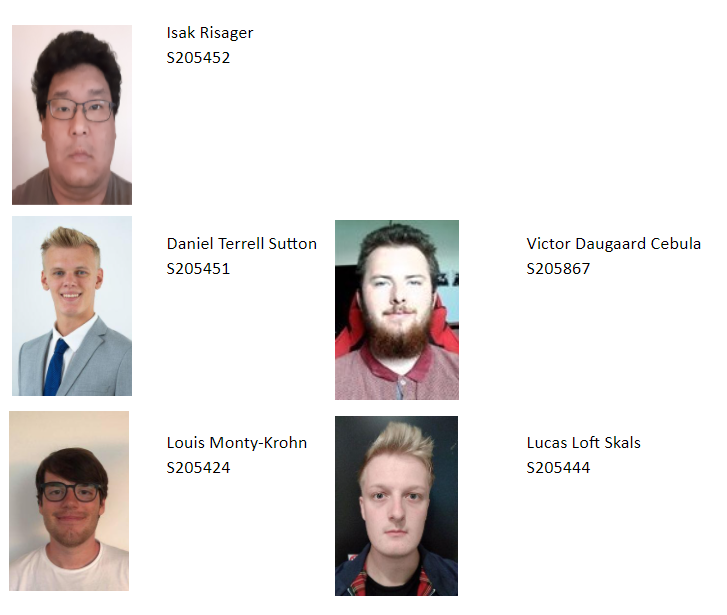
\includegraphics[width=0.9\textwidth]{Report/root/Forside.png}\\

\end{center}

18. Januar 2021

\vspace{0.1cm}

Gruppe 24

\vspace{0.3cm}

\url{https://github.com/louismonty/24_Final}
\end{center}
\end{titlepage}

\newpage
\begin{flushleft} % sætter tekststarten i venstre marginside.

\begin{center}
    \vspace{0.9cm}
    \textbf{Abstract}
\end{center}
\doublespacing

In the present project, we developed a Matador game based on Danish rulesets for Windows 10 home edition users. The project followed a Unified Process style of workflow including the following two phases: elaboration and construction. The analyses for the project included a requirements specification, use-case analysis and a domain analysis. The designs for the project included a system-sequence, sequence and design class analysis. The implementation resulted in a playable Matador game with no apparent errors or bugs. To reduce the risk of undetected bugs, JUnit tests were conducted for selected relevant software classes along with user tests for the entire program.



\end{flushleft}
\thispagestyle{fancy}

\newpage
\doublespacing
%\addcontentsline{toc}{section}{Table of Contents}
\renewcommand{\baselinestretch}{1}\normalsize
\tableofcontents
\renewcommand{\baselinestretch}{1}\normalsize
%\singlespacing
\thispagestyle{fancy} % force page style

\newpage
\section{Timeregnskab}
\centering
\begin{tabular}{ |c|c|c|c|c|c|  }
 \hline
 \multicolumn{6}{|c|}{Timeregnskab (timer)} \\
 \hline
 Aktivitet & Lucas & Victor & Louis & Daniel & Isak\\
 \hline
 
 
 Programmering      & 18 & 8 & 16 & 19 & 30 \\
 
 Møder              & 18 & 18 & 18 & 18 & 18 \\
 
 Rapportskrivning   & 12 & 6 & 3 & 3 & 3 \\
 
 \hline
 
 I alt              & 48 & 32 & 37 & 38 & 51 \\
 
 
 \hline
\end{tabular}
\thispagestyle{fancy}
\pagenumbering{arabic} 
\fancyfoot[C]{Page \thepage\ of \pageref{endOfDoc}}

\newpage
\section{Indledning}
\thispagestyle{fancy}
\begin{flushleft} % sætter tekststarten i venstre marginside.
\doublespacing

I dette projekt har vi arbejdet på, at udvikle en dansk version af spillet Matador ved brug af Java, hvor der er genbrugt visse kodedele fra CDIO del1 til CDIO del3, hvorend hensigtsmæssigt. Den nuværende version af Matadorspillet er udviklet ud fra et virkelig Matadorspils spilleregler, spillekort og spilleplade. Alle spillekort og spillepladen er implementeret, mens få spilleregler er udeladt.

\addlinespace

I projektet er der arbejdet iterativt efter en Unified Process style workflow. Dette vil sige, at der fra start af har været fokus på at implementere centrale use-cases, hvorefter der inkrementelt har været tilføjelser og revidering af use-cases. Derved er projektet altså udarbejdet i stil med en foreberedelses-, etablerings-, konstruktions- og overdragelsesfase (hhv. inception, elaboration, construction og transition på engelsk). Hertil er der udarbejdet analyser indenfor kravspecificering, use-cases, domænet og systemsekvenser. Designet er udviklet ved brug af sekvensdiagrammer og et klassediagram.
\addlinespace
Koden er skrevet ved hjælp af IntelliJ som udviklingsværktøj og Git som versionsstyringsværktøj. Herved er det sikret, at dokumentationen bliver opdateret tilsvarende det aktuelle Matador programs version. Yderligere har vi gjort brug af en Graphical User Interface (GUI), med tilhørende java bibliotek, som er blevet udleveret af kunden.
\addlinespace
I forbindelse med test af produktet er der i projektet udarbejdet JUnit tests og brugertests. Der er primært fokuseret på test, der måler funktionalitet af Matadorspillet.
\end{flushleft}

\newpage
\section{Projektplanlægning}
\input{Report/sources/09_Projektplanlægning}
\thispagestyle{fancy}

\newpage
\thispagestyle{fancy}
\section{Kravspecifikation}
\begin{flushleft}
\doublespacing
Vi har udbygget en prioriteret kravliste efter regelsættet der blev udleveret (se Figure \ref{MatadorRules1}-\ref{MatadorRules4} i bilag). Til det første møde med kunden (M1), blev der lavet en skitsering af kravlisten. Under dette møde med kunden blev kravlisten gennemgået, og sat i en prioriteret rækkefølge (se Figure \ref{Requirement list}). \\
\addlinespace[0.5cm]
Vi har nogle få punkter, der er valgt ikke at være med i spillet, grundet den begrænsede mængde tid til rådighed, og at de ikke var vigtige for funktionen eller glæden ved at spille spillet. Disse punkter inkluderer: (1) To måder at spille spillet på, en hurtig og normal måde, (2) at spillerne kan handle indbyrdes med skøder og løsladelseskort, (3) at en spiller bliver bank og auktionerer ejendomme fra spillere der er gået fallit og (4) at der er begrænsede antal huse og hoteller tilgængelige. Alle de fravalgte features vil senere kunne implementeres, hvis kunden ønsker det.  

\end{flushleft}
\begin{figure}[H]
    \centering
\begin{tabular}{ | c | c | } 
\hline
RS01 & En spiller kan købe grunde. \\ 
\hline
RS02 & Spillerne begynder på feltet START. \\ 
\hline
RS03 &  Der skal være en spilleplade på 40 felter.\\ 
\hline
RS04 &  Matadorspillet kan spilles af 2-6 spillere.\\ 
\hline
RS05 & Der skal være to terninger som begge har seks sider. \\
\hline
RS06 &  Hvis man slår to ens på terningerne rykker man og får lov til at kaste igen.\\ 
\hline
RS07 & For at komme ud af fængslet kan en spiller vælge mellem tre valgmuligheder:\\
& betal kaution, slå to ens eller brug løsladelseskort. \\ 
\hline
RS08 &Hver spiller starter med 30.000. \\ 
\hline
RS09 & Den spiller, der er sidst tilbage på spillepladen vinder. \\ 
\hline
RS10 & Hvis man lander på "Prøv lykken" feltet skal man trække et chancekort.\\
\hline
RS11 & Hvis en spiller skal betale mere end hvad spilleren har på kontoen,\\ & går spilleren fallit og ryger ud af spillet.\\
\hline
RS12 & En spiller rykker det antal øjne som terningerne viser på spillepladen. \\ 
\hline
RS13 & Vælger en spiller ikke at købe den grund, der landes på, \\
& sættes grunden på auktion.\\ 
\hline
RS14 & Hvis en spiller er i fængsel, kan spilleren ikke kræve husleje\\
& på de grunde, der er ejet af spilleren. \\
\hline
RS15 & Når man trækker et chancekort skal indholdet udføres med det samme. \\ 
\hline
RS16 &  Spillerne vælger indbyrdes, hvem der starter. \\%29
\hline
RS17 &  Hvis man ryger i fængsel modtager man ikke 4000 for at passere START.\\ 
\hline
RS18 & Det skal være muligt at ændre sprog i spillet.  \\ 
\hline
RS19 & Hvis man kaster to ens tre gange i træk ryger man i fængsel. \\
\hline
RS20 & Man kan købe huse/hotel, hvis man ejer alle grunde i tilsvarende farve. \\
\hline
RS21 &  Huslejen stiger, hvis der er bygget huse/hotel i forvejen.\\ 
\hline
RS22 &  Der må ikke være mere end et hus forskel mellem grunde af samme farve. \\ 
\hline
RS23 & For at opføre et hotel skal der være fire huse på grunden i forvejen.\\ 
\hline
RS24 & Der kan maksimum være et hotel per grund. \\ 
\hline
RS25 &Er man fængslet i tre omgange skal man i fjerde omgang betale 1000, \\
& hvorefter man bliver løsladt. \\
\hline
RS26 &  Kommer man ud af fængslet slår man  i samme tur med terningerne og rykker. \\ 
\hline
RS27 & Spillere kan pantsætte ubebyggede grunde for den pris, der står på skødet. \\
\hline
RS28 & Kommer man ud af fængslet ved at slå to ens, rykker man og får en ekstra tur.\\
\hline
RS29 & Der kræves ikke husleje på en pantsat grund.\\
\hline
RS30 & Lejen fordobles på en grund, hvis spilleren ejer alle grunde i samme farve.\\
\hline
RS31 & Når et hotel opføres gives husene tilbage til banken. \\%
\hline
\end{tabular}
\caption{Tabel over prioriterede krav}
\label{Requirement list}
\end{figure}


\newpage
\section{Analyse}
\begin{flushleft}
\subsection{Use-case diagram}
Vi startede med at lavet et use-case diagram, da dette er en central del af analysefase. Et use-case diagram viser det forskellige ting Player interagere med Matador spillet. Det diagram vi har udarbejdet kan man se at en Player kan "Play Matador", og til denne use-case er der nogle sub use-cases som er Start Game, Buy House or Hotel, Sell House or Hotel, Pawn Property, Buyback Pawned Property, Buy property or auction and Roll Dice. 
\begin{figure}[htp]
    \centering
    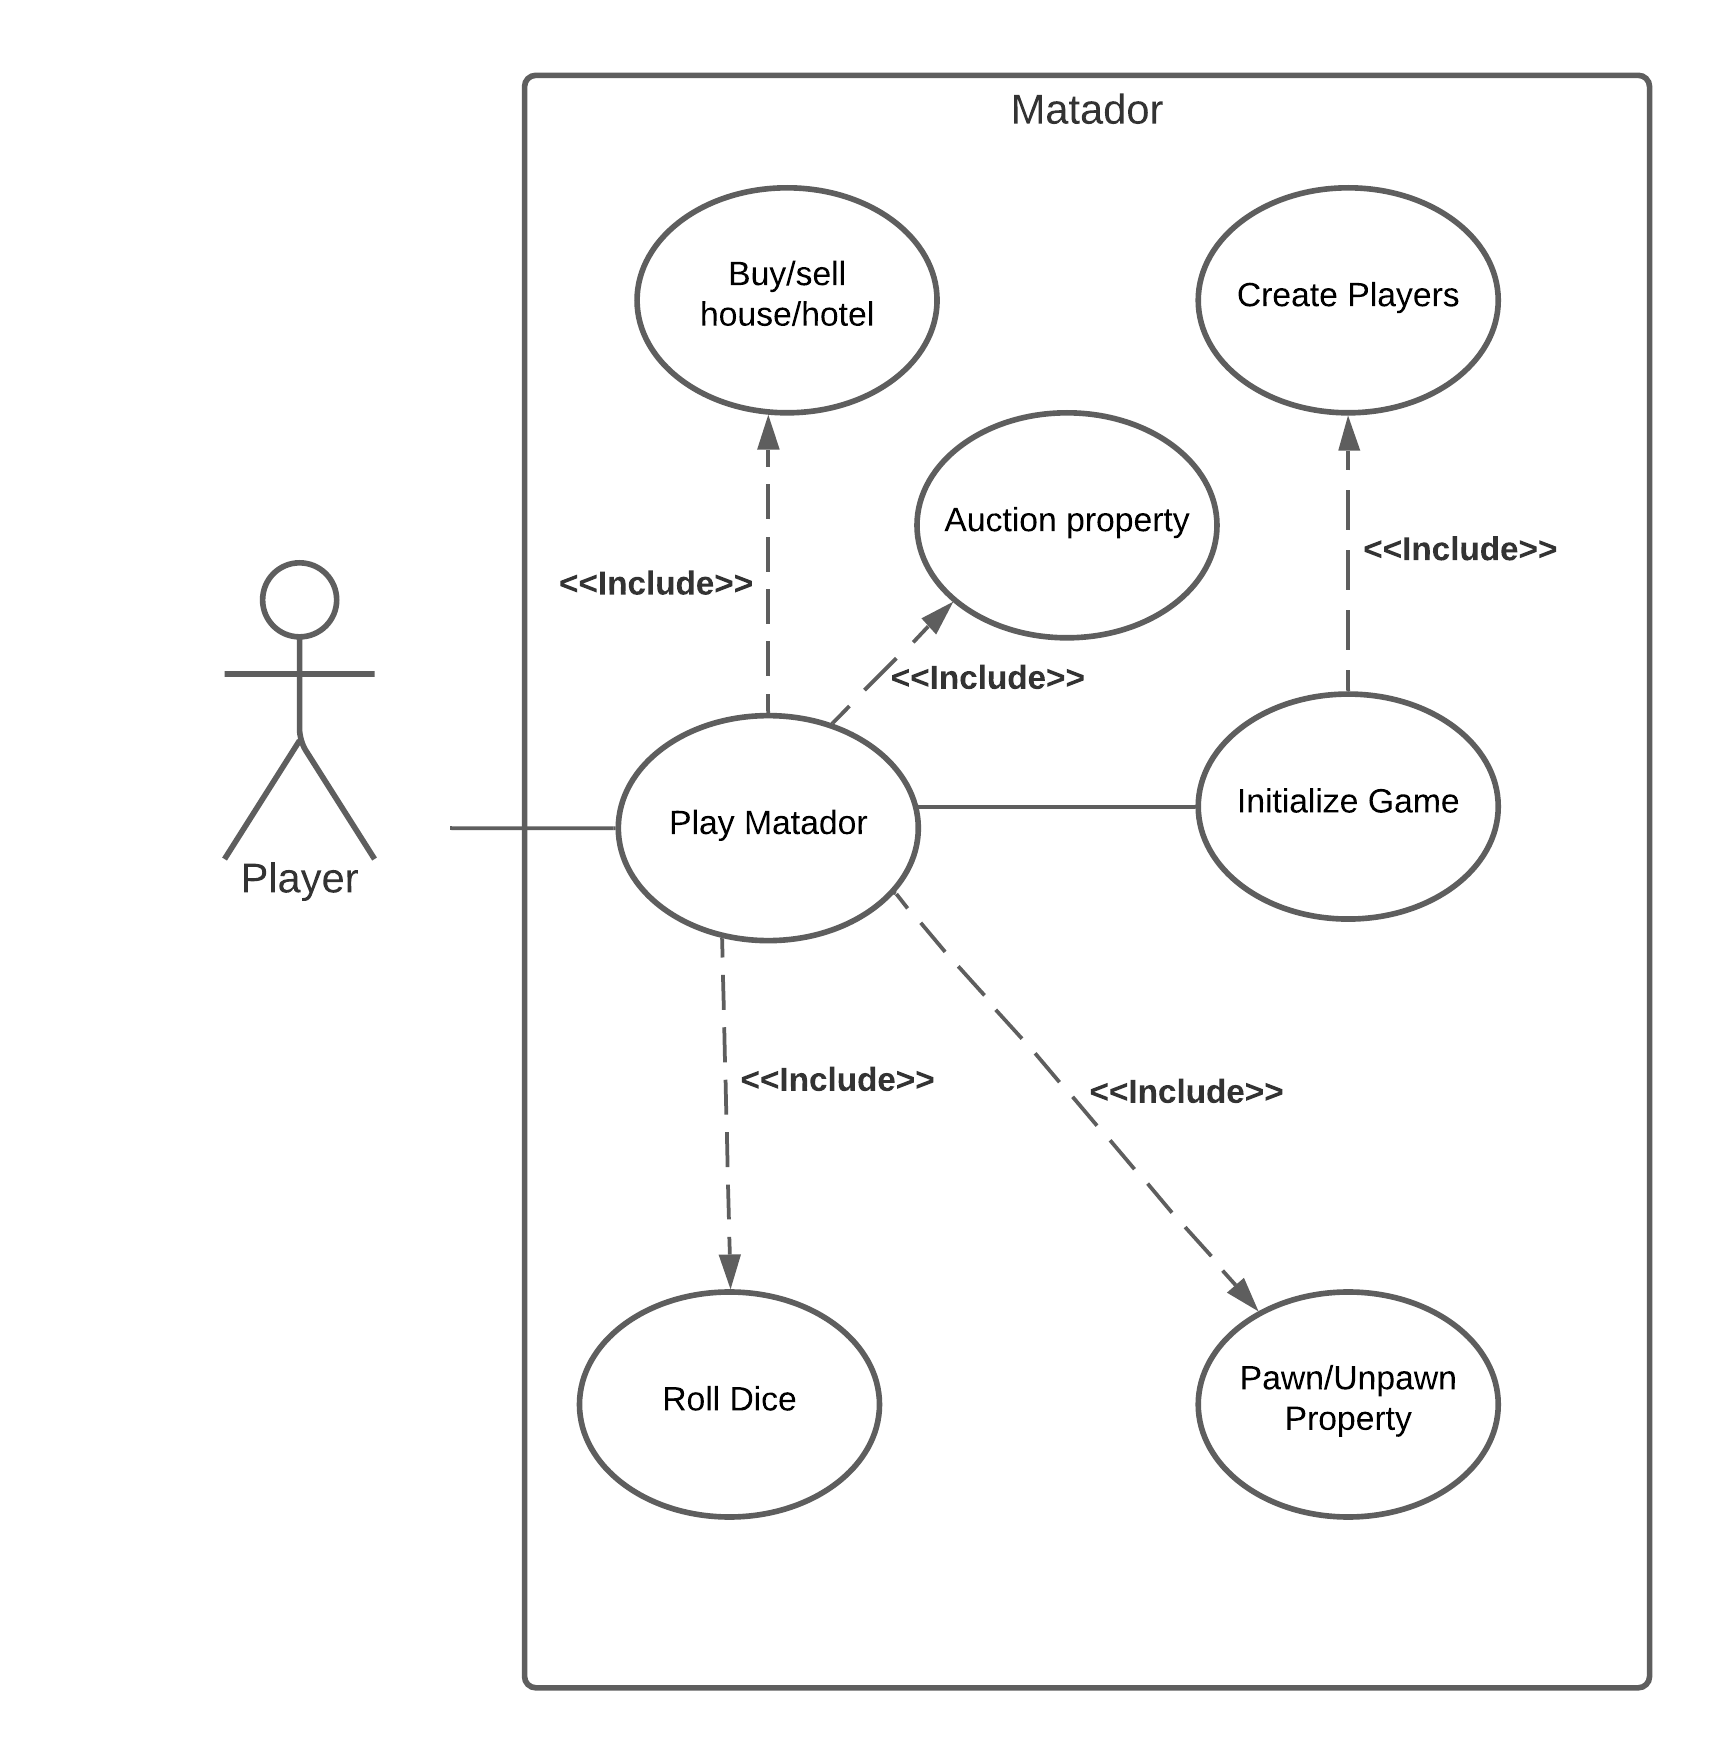
\includegraphics[width=12cm]{Report/figures/Use Case Diagram.png}
    \caption{Use-case diagram}
\end{figure}

\subsection{Central use-case: Roll dice}
Her under er en fully dressed beskrivelse af vores centrale use.case, Roll Dice. \\
\begin{figure}[htp]
    \centering
\begin{tabular}{ |c|c|c|c|c|c|  }
\hline
\multicolumn{2}{|c|}{Fully dressed use-case} \\
\hline
Use-case section & Comment \\
\hline
Use-case Name & Roll dice\\
\hline
Scope & Matador Game\\
\hline
Level & User Goal\\
\hline
Stakeholders and Interests & Players\\
\hline
Preconditions & Player chooses the GUI option to roll dice.\\
\hline
Postconditions & Game changes to next player.\\
\hline
Main success scenario & 1. Player rolls dice.\\
                      & 2. Dice values are shown on the GUI.\\
                    & 3. Player object moves on the GUI gameboard\\
                    & according to the sum of dice facevalue.\\
                    & 4. The gameboard field landed on \\
                    & executes its corresponding actions.\\
                    & 5. Current player's turn ends.\\
                    & 6. Game changes to next player.\\
\hline
Extensions & 6a. One player wins the game. \\
                   & 1. Winner is displayed.\\
                   & 2. Game exits.       \\
                   & 6b. A player rolls identical dices. \\
                   & 1. Steps 2 through 4 in Main success scenario\\
                   & are executed, but player can roll dice again. \\
                   & 1a. Player rolls identical dices thrice in a row.\\
                   & 1. Player moves to jail field on gameboard. \\
                   & 2. Continues from step 5 in Main success scenario.\\
\hline
Special Requirements & Arbitrary.\\
\hline
Technology and Data Variations list & N/A.\\
\hline
Frequency of Occurrence & Continuous.\\
\hline
Misc. & N/A.\\
\hline

    \end{tabular}\\
    \caption{Fully dressed use-case af roll dice use-case.}
\end{figure}
\doublespacing

\subsection{Sub use-cases}
Her er vores liste over use-cases.\\
\begin{figure}[htp]
    \centering
\begin{tabular}{ |c|c|c|c|c|c|  }
\hline
\multicolumn{2}{|c|}{Brief use-case} \\
\hline
Use-case & A short use case description \\
\hline
Start Game & Spillet starter med at man skal vælge \\
&hvor mange spiller der skal være med.\\
&Herefter indtaster hver spiller deres navn og den\\
&første spiller som indtaster deres navn starter.\\
\hline
Buy House or Hotel & I starten af spillerens tur får spilleren mulighed\\
&for at køber huse eller hoteller.\\
\hline
Sell House or Hotel & I starten af spillerens tur får spilleren mulighed\\
&for at sælge huse eller hoteller.\\
\hline
Pawn Property & Spilleren har mulighed for at pantsætte \\
&sine grunde i starten af turen.\\
\hline
Buyback Pawned Property & Spilleren har mulighed for at tilbage købe\\
&pantsætte grunde i starten af turen.\\
\hline
Buy Property or Auction & Hvis man lander på en grund for man \\
&mulighed for at købe den, men hvis man ikke\\
&gider eller kan købe grunden bilver den\\
&sat til salg på aution hvor alle kan deltage\\
\hline


    \end{tabular} \\
    \caption{Brief use-cases}
\end{figure}
\doublespacing


\subsection{Domæne model}
Det centrale objekt i domæne modelen er MatadorGame. Det indholder mellem 2 til 6 Player, 46 ChanceCard, 2 Dice og en Field. Til hver Player som bliver opretter bliver der også oprettet en Account, som bliver påvirket af Field. Field har også JailField, ChanceField, CustomField, PropertyField, StartField, TaxField, SodaField and FerryField.
\begin{figure}[htp]
    \centering
    \includegraphics[width=16cm]{Report/figures/Domæne model.png}
    \caption{Domæne model}
\end{figure}

\subsection{Systemsekvensdiagram}
Her til at afrund vores analysedel hvor vi har udarbejdet et systemsekvensdiagram over Matador spillet. Systemsekvensdiagram viser Player og interaktion med Matador spillet. 
\begin{figure}[htp]
    \centering
    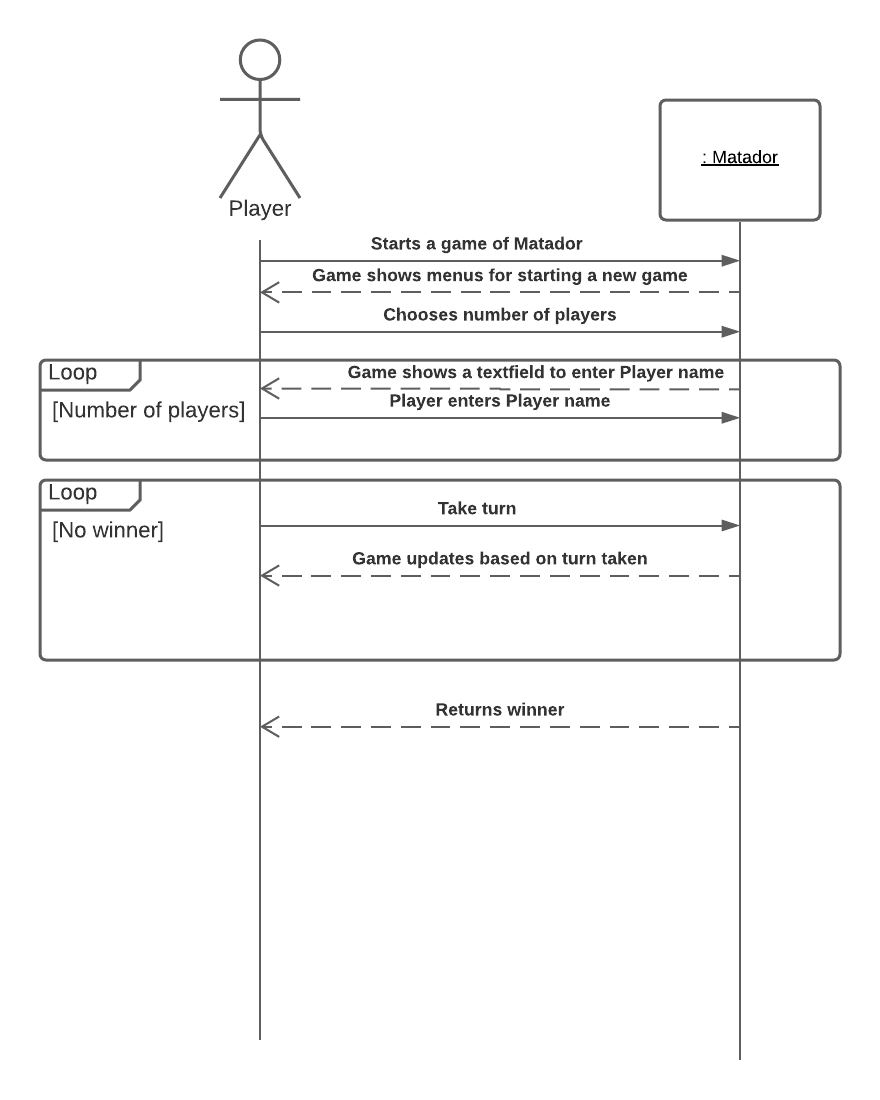
\includegraphics[width=13cm]{Report/figures/System Sekvens Diagram.png}
    \caption{Systemsekvensdiagram}
\end{figure}

\end{flushleft}
\thispagestyle{fancy}

\newpage
\section{Design}
\begin{flushleft}
\doublespacing
Til dette projekt har vi valgt at designe vores program efter GRASP princippper. Herved har vi stilet efter, at vores spil har lav kobling, høj samhørighed, polymorphism, creators og information experts. Hertil er designet to sekvensdiagrammer, der viser en oversigt af objektkald for UC01: Roll dice og UC04: Buy/sell house/hotel (se Figure 
\subsection{Sekvensdiagrammer}

\begin{figure}[htp]
    \centering
    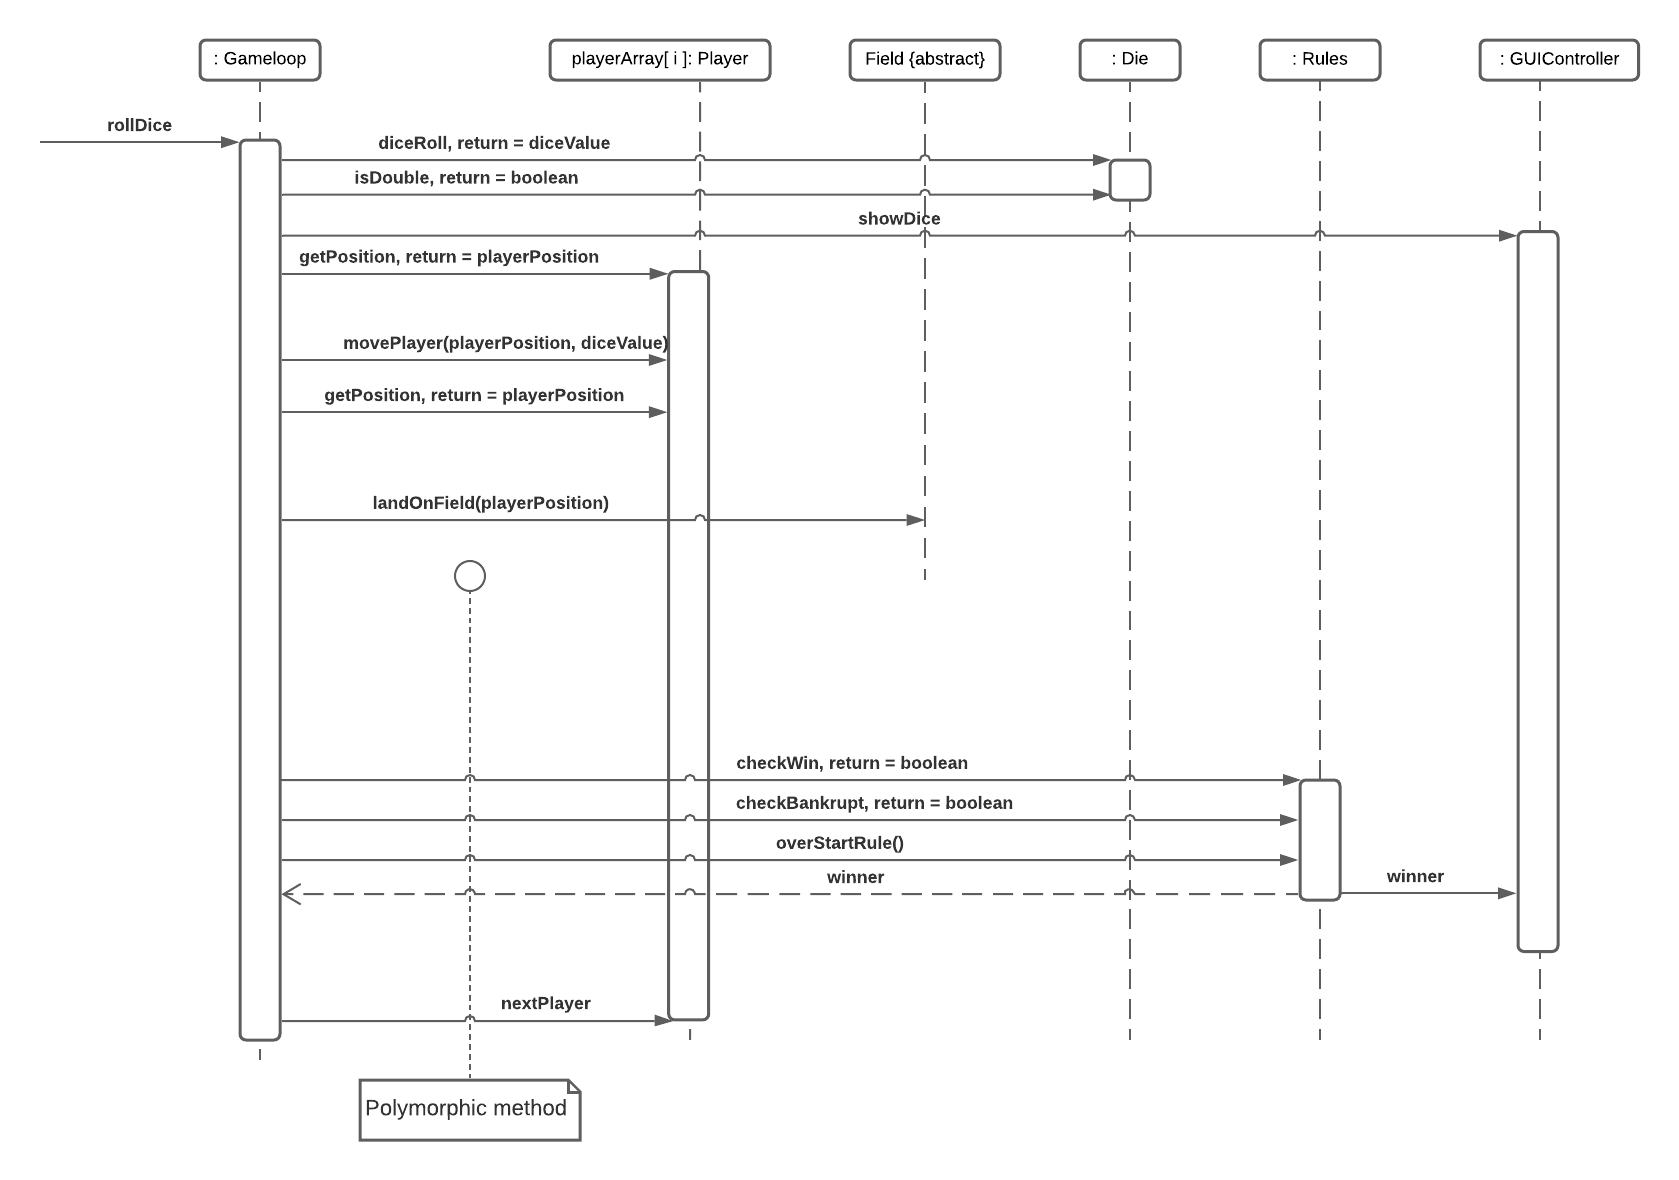
\includegraphics[width=13cm]{Report/figures/Roll Dice Sekvensdiagram.png}
    \caption{Sekvensdiagram over roll dice use-case.}
\end{figure}
\begin{figure}[htp]
    \centering
    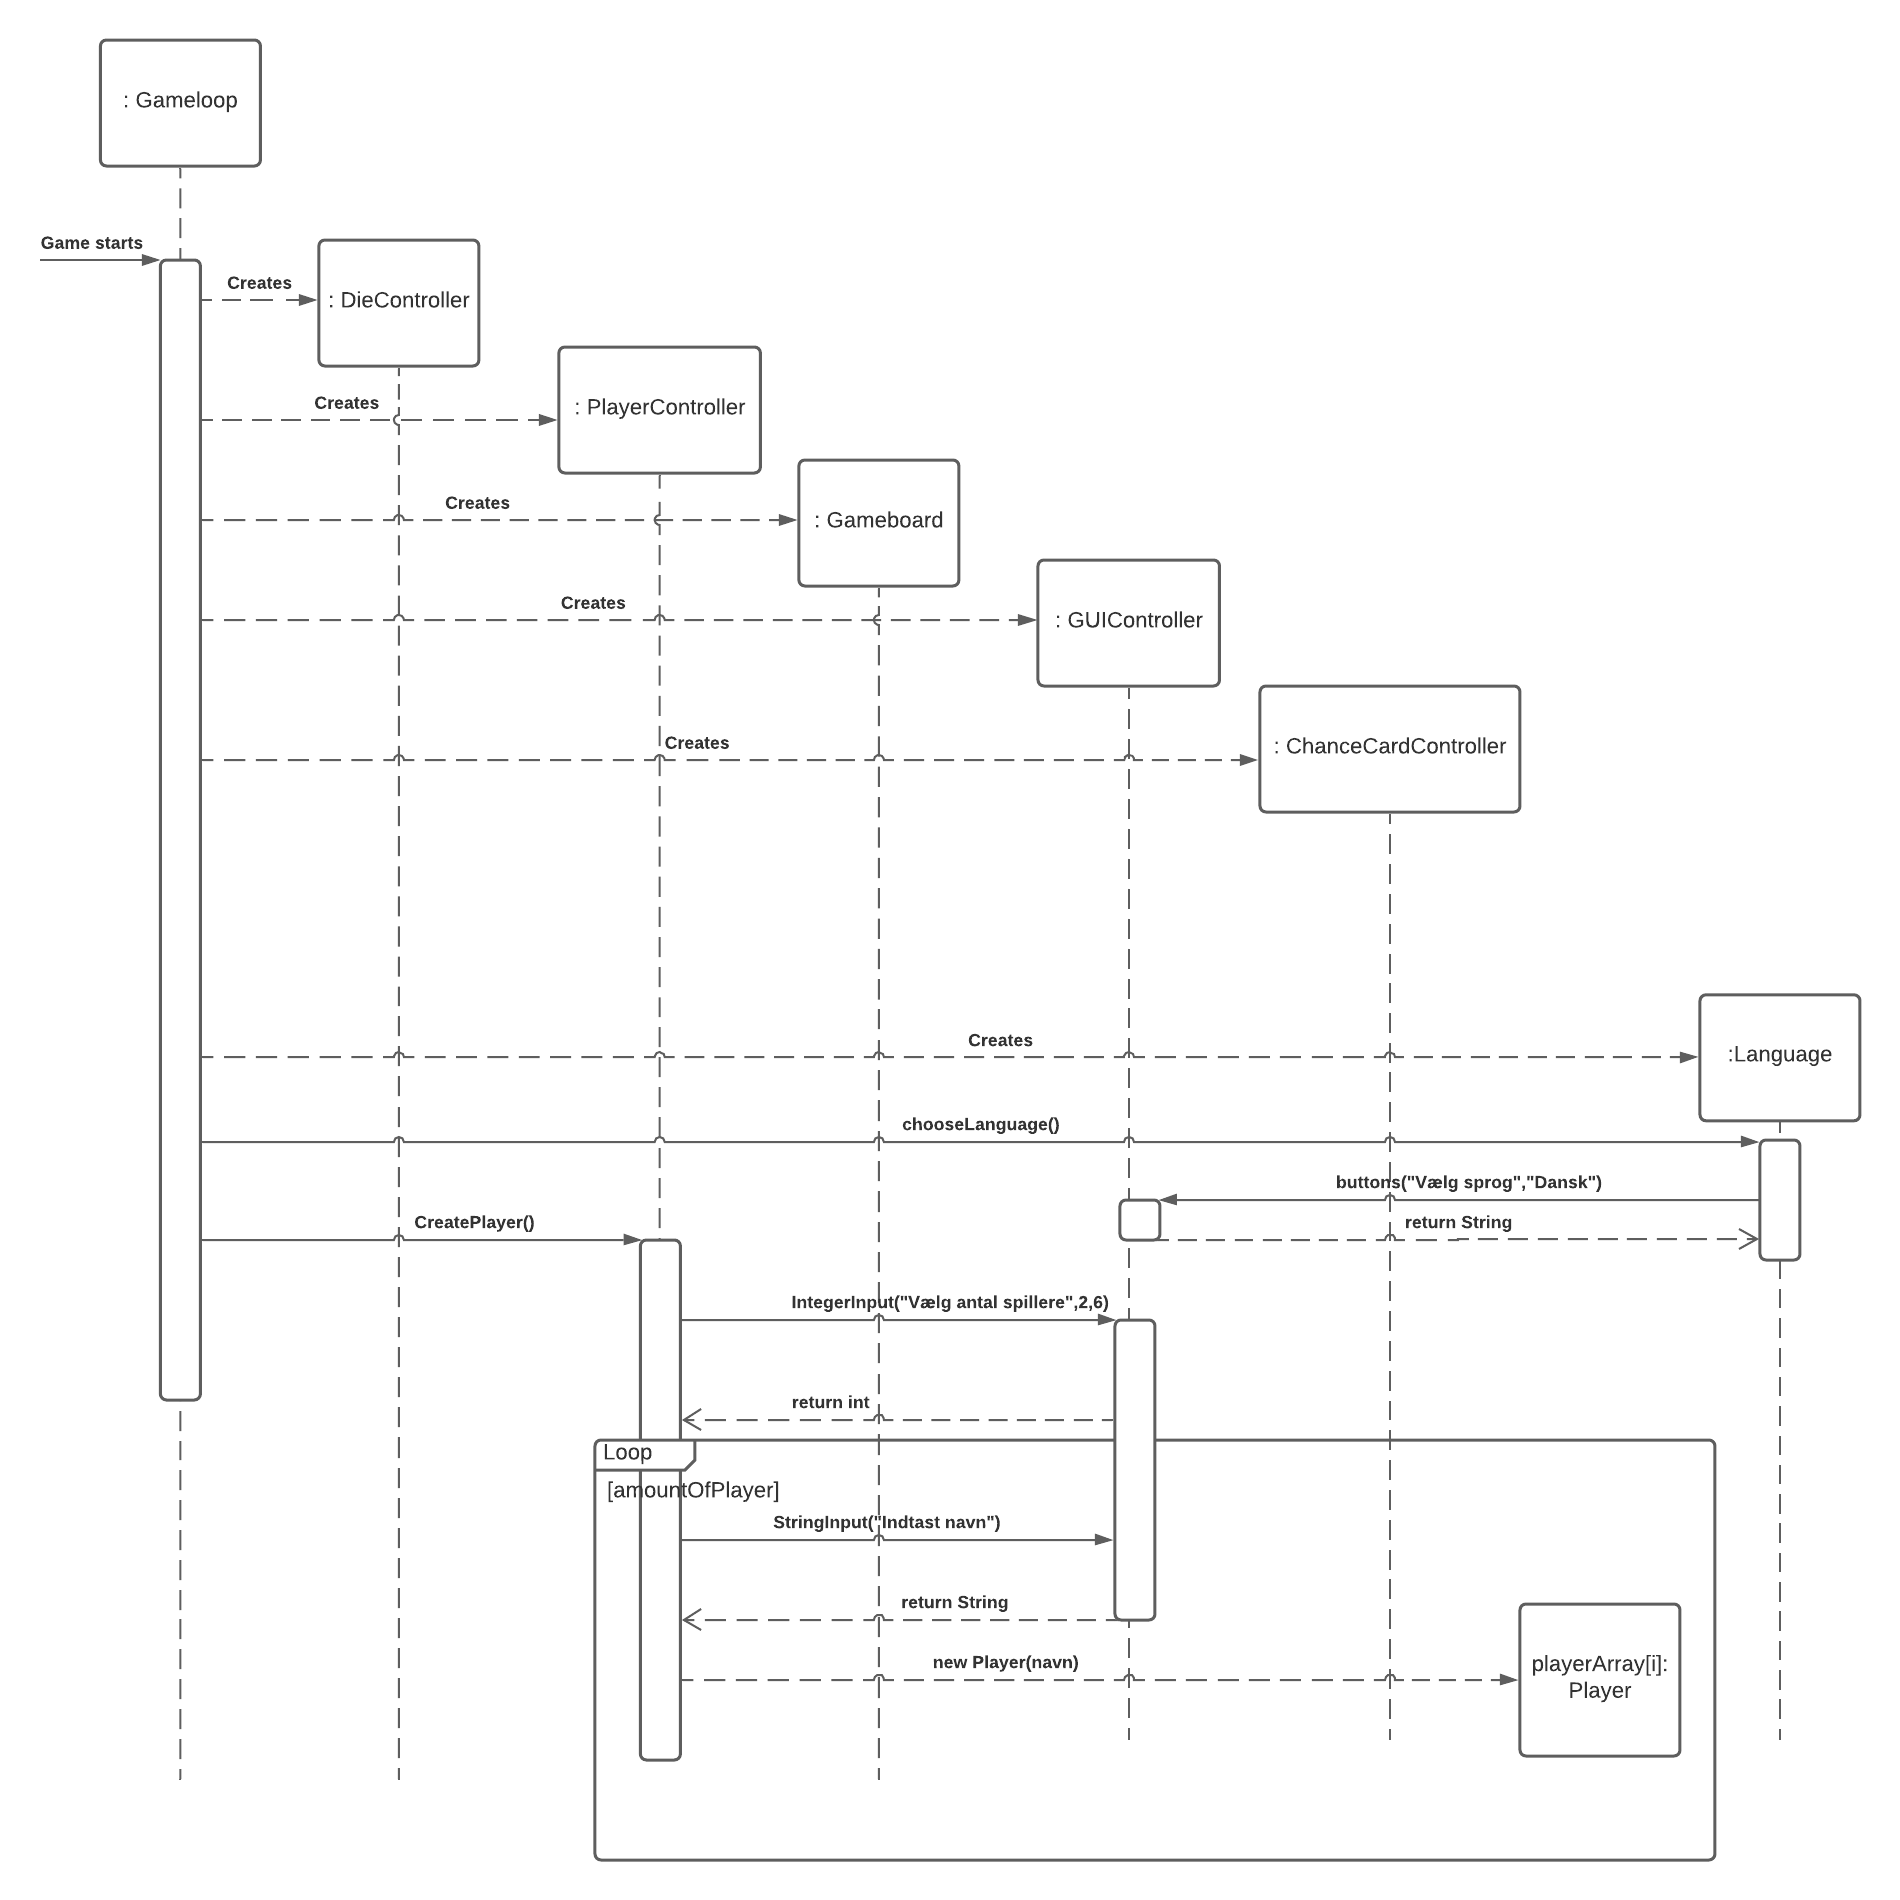
\includegraphics[width=13cm]{Report/figures/Start Game Sekvensdiagram.png}
    \caption{Sekvensdiagram over start game use-case.}
\end{figure}

\subsection{Klassediagram}

\end{flushleft}
\thispagestyle{fancy}

\newpage
\section{Implementering}
\begin{flushleft}
\doublespacing

\subsection{Chancecard - hjælpemetoder}
Da chancekortene(Prøv Lykken kort) arbejder indenfor forskellige kategorier, har vi valgt at opdele dem i IncomeChanceCard, JailChanceCard, MoveChanceCard og PaymentChanceCard klasser. Vi skal have et dæk der kan bruge metoderne fra alle klasserne, så derfor har vi en overordnet klasse der hedder ChanceCard, som alle de nævnte chancekortsklasser nedarver fra. Da de kun nedarver en variabel, har vi valgt at snakke mere om nedarvning i det næste afsnit. I stedet vil vi se på hjælpemetoder der bliver brugt i chancekort klasserne. Da klasserne arbejder indenfor en kategori, har alle metoder i hver klasse en tætlignede funktion. I IncomeChanceCard modtager spilleren et beløb, i MoveChanceCard flytter spilleren position osv. Derfor er der implementeret hjælpemetoder for, at undgå for meget kodereplikation.
Som eksempel vil vi se på IncomeChanceCard. Her har vi lavet to hjælpemetoder. addBalanceFromCard tilføjer penge til spillerens konto, mens receiveMoneyFromOthers giver spilleren et beløb fra hver spiller. De resterende metoder i klasser benytter én af de to hjælpemetoder.
Det kan ses i Figure \ref{IncomeChanceCard assist methods}, at metoderne lotteryCard og stockDividendsCard benytter sig af hjælpemetoden addBalanceFromCard.

\begin{figure}[H] %brug begin{figure} til alle figurer.
    \centering
    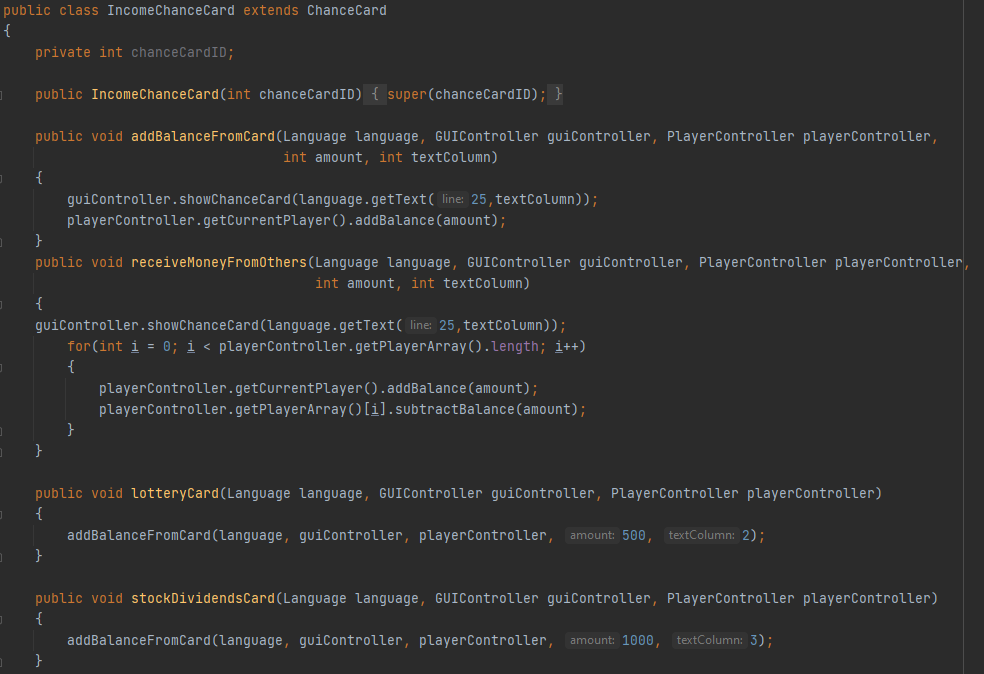
\includegraphics[width=14cm]{Report/figures/Codesections/IncomeChanceCard_addBalanceFromCard()+receiveMoneyFromOthers().PNG}
    \caption{Hjælpemetoder i IncomeChanceCard}
    \label{IncomeChanceCard assist methods}
\end{figure}


\subsection{Fields - nedarvning og polymorphism}
I Field klassen (se Figure \ref{Field_constructor}) har vi gjort klassen abstract, så der ikke kan dannes objekter af klassen, men kun af nedarvede klasser for Field. Vi bruger protected som access modifier for instansvariablerne, så de kan tilgås af nedarvede klasser.
\begin{figure}[H] %brug begin{figure} til alle figurer.
    \centering
    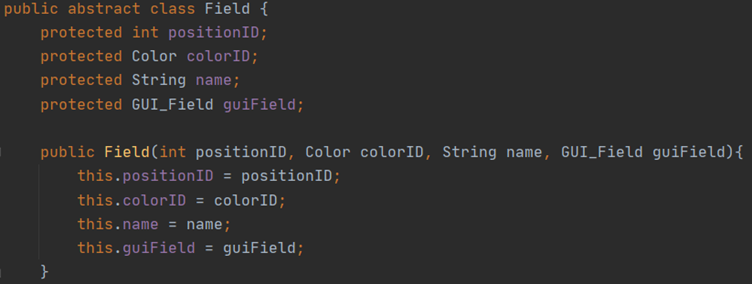
\includegraphics[width=14cm]{Report/figures/Codesections/Field_constructor().png}
    \caption{Field klassens konstruktør}
    \label{Field_constructor}
\end{figure}

I BuyableField klassen det ses, at klassen nedarver fra Field klassen (se Figure \ref{BuyableField_constructor}). Her bruges super() variable til at referere til objekt instanser fra dens parent class, Field. Det ses yderligere, at vi igen bruger abstract klassen - dette er fordi BuyableField er yderligere nedarvet af flere klasser, hvor vi ikke ønsker, at der kan laves objekter direkte af BuyableField.
    
\begin{figure}[H]
    \centering
    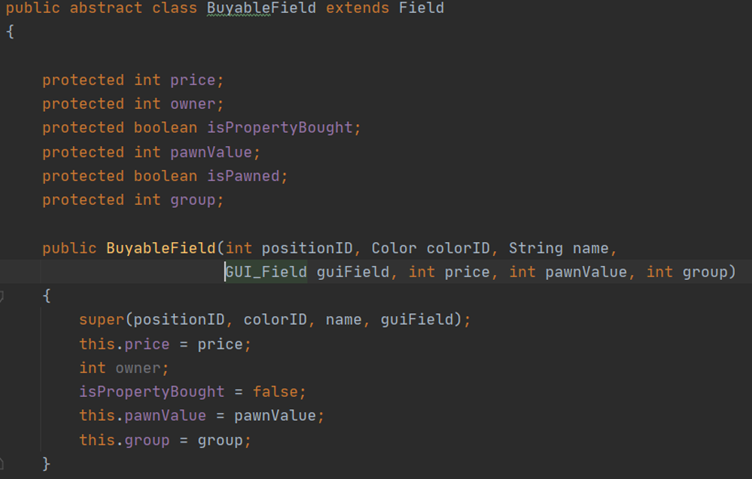
\includegraphics[width=14cm]{Report/figures/Codesections/BuyableField_constructor().png}
    \caption{BuyableField klassens konstruktør}
    \label{BuyableField_constructor}
\end{figure}

I Field klassen ses det yderligere, at der findes an abstract metode, landOnField() (se Figure \ref{Field_landOnField}). Dette vil sige, at metoden skal defineres i de nedarvede klasser af Field og ikke indeholder en body, da denne specificeres af de nedarvede klasser.

\begin{figure}[H]
    \centering
    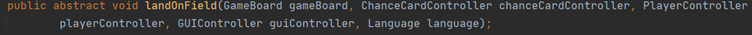
\includegraphics[width=14cm]{Report/figures/Codesections/Field_landOnField().png}
    \caption{Field klassens landOnField() metode}
    \label{Field_landOnField}
\end{figure}

I JailField klassen kan man se et eksempel på polymorphism af metoden landOnField(), som er nedarvet fra Field klassen. Herved bliver logikken i landOnField() anderledes i JailField klassen fra sine sibling-classes. 
    
\begin{figure}[H]
    \centering
    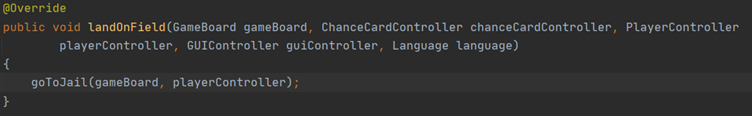
\includegraphics[width=14cm]{Report/figures/Codesections/BuyAbleField_landOnField().png}
    \caption{JailField klassens landOnField() metode}
    \label{Jailfield_landOnField}
\end{figure}

\subsection{Language - 2D array, tekstfil og try/catch}
Language klassen bruges til at indlæse Strings fra en csv fil et 2D array, hvor linjetallet i csv filen bliver indlæst i første dimension af String[][] ImportedText mens String objekterne bliver indlæst i anden dimension af ImportedText. Herved sikrer vi os, at det er nemt at ændre i tekstfilen og lave andre versioner af den - f.eks. hvis man ønsker at oversætte hele tekstfilen til et andet sprog. Yderligere bruger vi try/catch statements til at udskrive en error, hvis filen ikke bliver fundet. For at hente teksten, der bliver indlæst fra filen, kan man bruge metoden getText, hvor der indsættes to heltal som parametre, der svarer til hhv. linjen og kolonnen i csv filen.
\begin{figure}[htp] %brug begin{figure} til alle figurer.
    \centering
    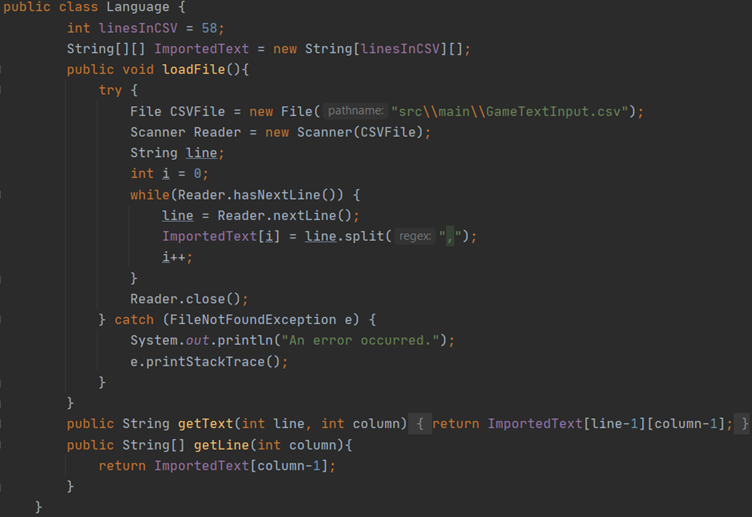
\includegraphics[width=14cm]{Report/figures/Codesections/Language_Language.png}
    \caption{Oversigt af Language klassen}
    \label{LanguageKlasse}
\end{figure}

\subsection{Menu - instanceOf og expandable array}
I klassen Menu, er der lavet metoderne expandArr og expandStrArr. Disse to metoder udvider et modtaget array med én. Dermed har vi mulighed for at udvide arrays. Når der skal ses hvilke grunde der kan købes huse elller hotel på, og hvilke man ejer og kan pantsætte osv. kan man gå alle felterne igennem, og hver gang man finder en felt der matcher ens beskrivelse, da tilføje dem til et array der bliver én større for hver gang (se Figure \ref{Expanding arrays}).

\begin{figure}[H] %brug begin{figure} til alle figurer.
    \centering
    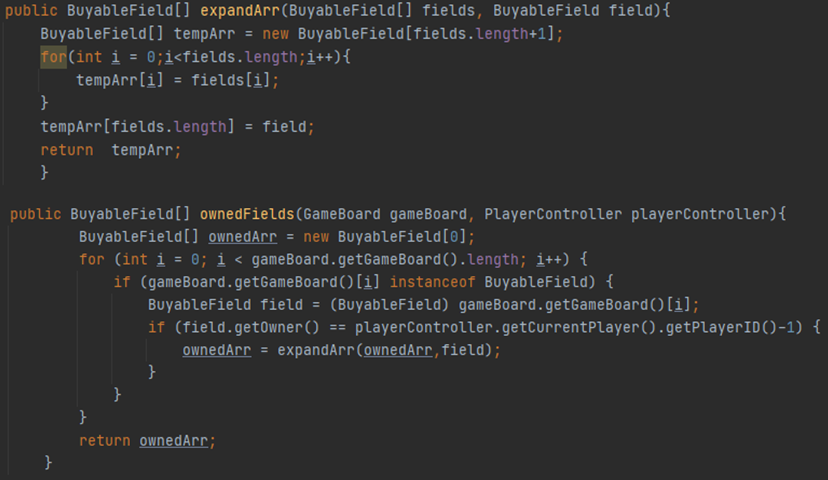
\includegraphics[width=14cm]{Report/figures/Codesections/Menu_expandArr()+ownedFields().PNG}
    \caption{Metoderne expandArr og ownedFields der benytter expandArr}
    \label{Expanding arrays}
\end{figure}


\end{flushleft}{}
\thispagestyle{fancy}

\newpage
\section{Test}
\begin{flushleft}
\doublespacing

\subsection{JUnit tests}
\subsection{Brugertest}

\begin{figure}[htp] %brug begin{figure} til alle figurer.
    \centering
    
\includegraphics[width=14cm]{Report/figures/Usertests/TC01.png}
    \caption{Tabel over TC01}
    \label{Testcase01}
\end{figure}

\begin{figure}[htp] %brug begin{figure} til alle figurer.
    \centering
    
\includegraphics[width=14cm]{Report/figures/Usertests/TC02.png}
    \caption{Tabel over TC02}
    \label{Testcase02}
\end{figure}

\begin{figure}[htp] %brug begin{figure} til alle figurer.
    \centering
    
\includegraphics[width=14cm]{Report/figures/Usertests/TC03.png}
    \caption{Tabel over TC03}
    \label{Testcase03}
\end{figure}

\end{flushleft}
\thispagestyle{fancy}

\newpage
\begin{flushleft}
\section{Konklusion og bemærkninger}
\begin{flushleft}
\doublespacing

I det foreværende projekt, CDIO Final, har vi udarbejdet et virtuelt Matadorspil udviklet i Java. Vi har gennemført projektet ud fra en ambitiøs kravspecifikation og har haft fokus på at levere et program der virker. Det lykkedes, da alle implementerede dele af spillet virker, og som beskrevet i afsnittet om kravspecifikatiner har vi kun fravalgt få features i forhold til spillereglerne. \\\

I CDIO del3 udviklede vi et Junior Monopoly. Arkitekturen fra dette projekt har vi videreudviklet på. Eksempelvis er der ændret på strukturen omkring GUI håndtering. Vi har udviklet en dansksproget udgave, men har inkluderet muligheden for nemt, at erstatte tekster med eventuelle oversatte varianter. Således vil spillet hurtigt kunne leveres til andre lande i andre sprog.\\\

Vi har anvendt mange af de programkonstruktioner, som der er blevet gennemgået igennem semestret og har haft fokus på, at klasserne nedarver mest muligt fra hinanden, at gøre koden overskuelig at læse og lave metoder der kan genbruges. Dog ville vi, som beskrevet i design afsnittet, i en fremtidig version sørge for at minimere dependencies og dermed opnå lavere kobling.\\\

Når vi ser tilbage, oplever vi, at vores planlægning i store træk blev fulgt ret godt i løbet af processen.
Alt i alt har vi som gruppe leveret en ambitiøs og velfungerende virtuel udgave af Matadorspillet, der opfylder alle de krav, der blev sat sammen med kunden.




\end{flushleft}
\end{flushleft}
\thispagestyle{fancy}

\newpage
\begin{flushleft}
\section{Tegn og ordforklaring}
\end{flushleft}
\begin{flushleft}
\begin{figure}[htp]
    \centering
\begin{tabular}{ | c | c | } 
\hline
Tegn / ord & Forklaring \\ 
\hline
UTF-8 & Indkodning af unicode tegnsættet for at kunne visualisere symboler. \\ 
\hline
IntelliJ & IDE, der understøttet flere forskellige programmeringssprog, inkl. Java. \\ 
\hline
Git & Versionsstyringsværktøj. \\ 
\hline
Overleaf & Online tekstredigeringsværktøj, der følger LaTeX framework. \\ 
\hline
Maven & Værktøj til at organisere java-projekter og tests. \\ 
\hline
JUnit & Framework til at teste forskellige units i Java. \\ 
\hline
GUI & Graphical User Interface: Den visuelle del af programmet. \\ 
\hline
GRASP & Et design pattern. Står for General Responsibility Assignment Software Patterns \\
\hline
 
\hline
\end{tabular}
\caption{Tabel Ordforklaring}
\end{figure}

\end{flushleft}
\thispagestyle{fancy}

\newpage
\begin{flushleft}
\section{Bilag}
\begin{flushleft}
\subsection{Kildekode indholdsfortegnelse}
\subsection{Brugertests}
\begin{figure}[H] %brug begin{figure} til alle figurer.
    \centering
    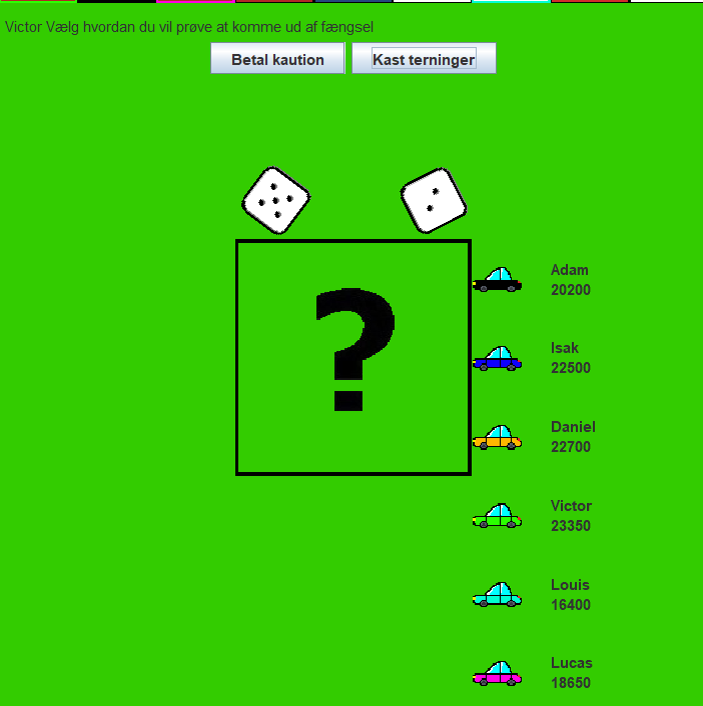
\includegraphics[width=16cm]{Report/figures/Usertests/BilagTC01.png}
    \caption{TC01 Screenshot}
    \label{TC01Bilag}
\end{figure}\begin{figure}[H] %brug begin{figure} til alle figurer.
    \centering
    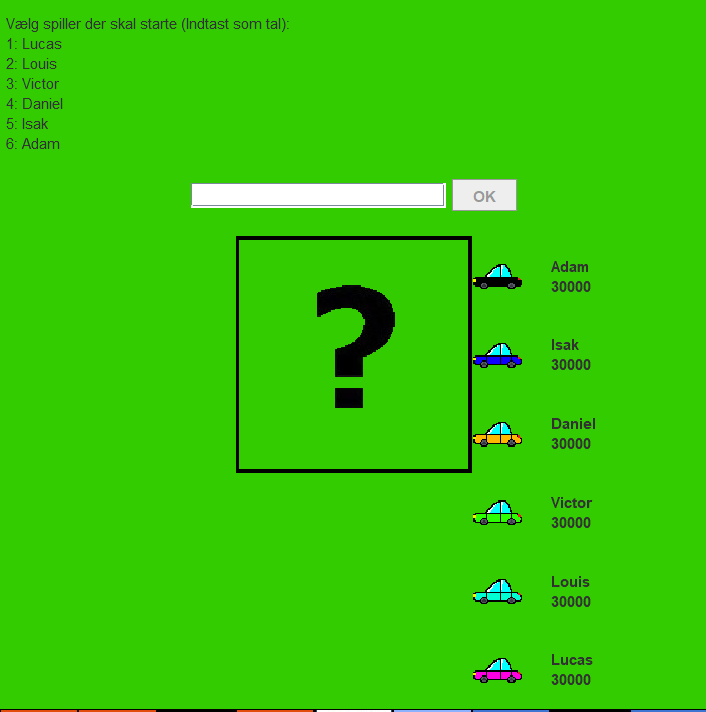
\includegraphics[width=16cm]{Report/figures/Usertests/BilagTC02.png}
    \caption{TC02 Screenshot}
    \label{TC02Bilag}
\end{figure}\begin{figure}[H] %brug begin{figure} til alle figurer.
    \centering
    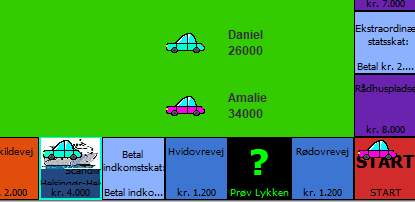
\includegraphics[width=16cm]{Report/figures/Usertests/BilagTC03.png}
    \caption{TC03 Screenshot}
    \label{TC03Bilag}
\end{figure}
\end{flushleft}

\label{endOfDoc}
\end{flushleft}
\label{endOfDoc}
\end{document}